\documentclass[border=10pt]{standalone}
\usepackage{ctex}
\usepackage{amsmath,amssymb,bm}
\usepackage{tikz}
\usepackage{tikz-feynman}
\tikzfeynmanset{compat=1.1.0}
\usetikzlibrary{positioning,arrows.meta,shapes.geometric,fit,backgrounds,calc}

\tikzset{
  stepbox/.style={
    draw=#1, fill=#1!6, rounded corners=5pt,
    minimum width=14cm, align=left, font=\small, inner sep=8pt
  },
  stepbox/.default=blue,
  stepnum/.style={circle, draw=#1, fill=#1!20, font=\bfseries\small, inner sep=3pt, minimum size=0.6cm},
  stepnum/.default=blue,
  integralvar/.style={font=\scriptsize\ttfamily, text=red!80!black},
  equiv/.style={font=\scriptsize, text=green!60!black},
}

\begin{document}
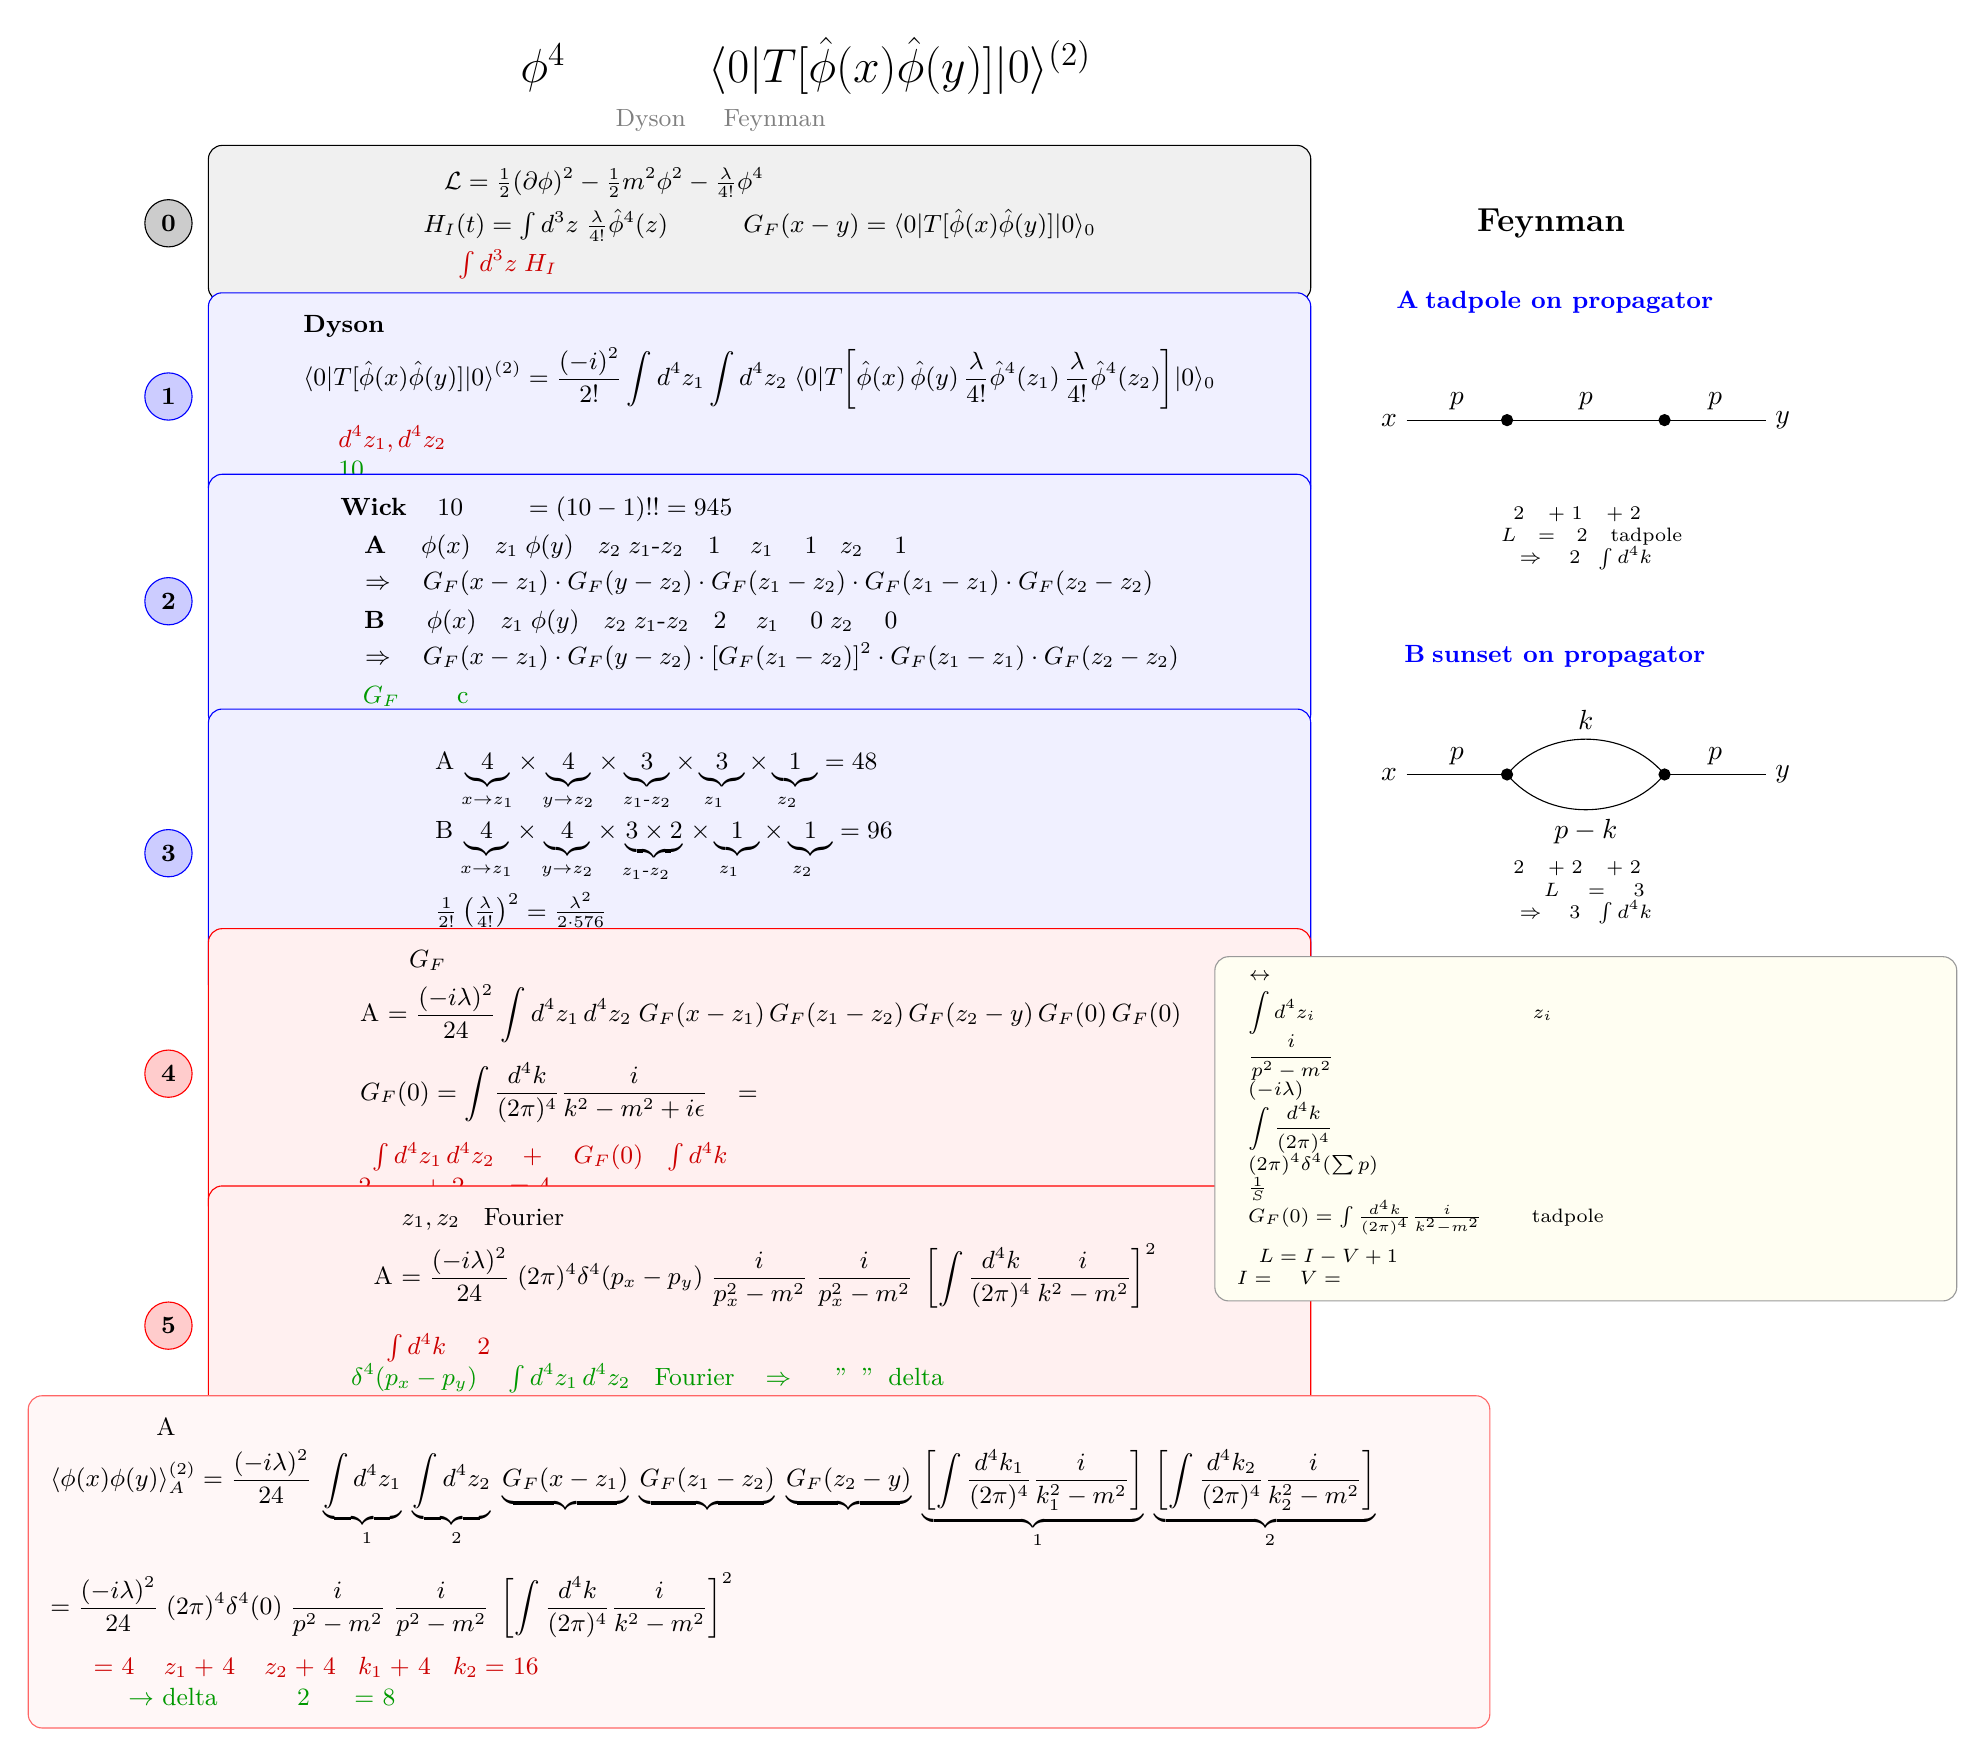
\begin{tikzpicture}[node distance=0.6cm]

% ============================================================
% TITLE
% ============================================================
\node[font=\LARGE\bfseries] (title) at (0, 0) {完整代入示例：$\phi^4$ 理论二阶两点函数 $\langle 0\vert T[\hat\phi(x)\hat\phi(y)]\vert 0\rangle^{(2)}$};
\node[font=\small, text=gray] at (0, -0.7) {展示从 Dyson 级数到 Feynman 图的每一步公式，标注积分变量};

% ============================================================
% STEP 0: Setup
% ============================================================
\node[stepnum=black] (n0) at (-7.5, -2) {0};
\node[stepbox=black, anchor=west] (s0) at (-7, -2) {%
  \textbf{设定}：$\mathcal{L} = \frac{1}{2}(\partial\phi)^2 - \frac{1}{2}m^2\phi^2 - \frac{\lambda}{4!}\phi^4$\\[3pt]
  $H_I(t) = \int d^3z\;\frac{\lambda}{4!}\hat\phi^4(z)$，\quad 自由传播子 $G_F(x-y) = \langle 0\vert T[\hat\phi(x)\hat\phi(y)]\vert 0\rangle_0$\\[3pt]
  \textcolor{red!80!black}{积分变量：$\int d^3z$（$H_I$ 的空间积分）}
};

% ============================================================
% STEP 1: Dyson expansion
% ============================================================
\node[stepnum=blue] (n1) at (-7.5, -4.2) {1};
\node[stepbox=blue, anchor=west] (s1) at (-7, -4.2) {%
  \textbf{Dyson 展开到二阶}：\\[3pt]
  $\displaystyle\langle 0\vert T[\hat\phi(x)\hat\phi(y)]\vert 0\rangle^{(2)} = \frac{(-i)^2}{2!}\int d^4z_1\int d^4z_2\;\langle 0\vert T\!\left[\hat\phi(x)\,\hat\phi(y)\,\frac{\lambda}{4!}\hat\phi^4(z_1)\,\frac{\lambda}{4!}\hat\phi^4(z_2)\right]\!\vert 0\rangle_0$\\[5pt]
  \textcolor{red!80!black}{积分变量：$d^4z_1, d^4z_2$（两个顶点的时空坐标）}\\
  \textcolor{green!60!black}{被积函数：10 个场算符的编时真空期望}
};

% ============================================================
% STEP 2: Wick theorem
% ============================================================
\node[stepnum=blue] (n2) at (-7.5, -6.8) {2};
\node[stepbox=blue, anchor=west] (s2) at (-7, -6.8) {%
  \textbf{Wick 定理}：10 个场的完全收缩 $= (10-1)!! = 945$ 项。按拓扑分类，取连通贡献：\\[3pt]
  \textbf{类型 A}（树图）：$\phi(x)$ 连 $z_1$，$\phi(y)$ 连 $z_2$，$z_1$-$z_2$ 间 1 条线，$z_1$ 自环 1 条，$z_2$ 自环 1 条\\[2pt]
  $\quad\Rightarrow\quad G_F(x-z_1)\cdot G_F(y-z_2)\cdot G_F(z_1-z_2)\cdot G_F(z_1-z_1)\cdot G_F(z_2-z_2)$\\[3pt]
  \textbf{类型 B}（一圈图）：$\phi(x)$ 连 $z_1$，$\phi(y)$ 连 $z_2$，$z_1$-$z_2$ 间 2 条线，$z_1$ 自环 0，$z_2$ 自环 0\\[2pt]
  $\quad\Rightarrow\quad G_F(x-z_1)\cdot G_F(y-z_2)\cdot [G_F(z_1-z_2)]^2\cdot G_F(z_1-z_1)\cdot G_F(z_2-z_2)$\\[3pt]
  \textcolor{green!60!black}{每个 $G_F$ 都是已知函数（c 数），此步无新积分}
};

% ============================================================
% STEP 3: Combinatorial factors
% ============================================================
\node[stepnum=blue] (n3) at (-7.5, -10) {3};
\node[stepbox=blue, anchor=west] (s3) at (-7, -10) {%
  \textbf{组合因子}（收缩方式计数）：\\[3pt]
  类型 A：$\underbrace{4}_{x\to z_1}\times\underbrace{4}_{y\to z_2}\times\underbrace{3}_{z_1\text{-}z_2}\times\underbrace{3}_{z_1\text{ 自环}}\times\underbrace{1}_{z_2\text{ 自环}} = 48$\\[3pt]
  类型 B：$\underbrace{4}_{x\to z_1}\times\underbrace{4}_{y\to z_2}\times\underbrace{3\times 2}_{z_1\text{-}z_2\text{ 两条}}\times\underbrace{1}_{z_1\text{ 自环}}\times\underbrace{1}_{z_2\text{ 自环}} = 96$\\[3pt]
  乘以 $\frac{1}{2!}\left(\frac{\lambda}{4!}\right)^2 = \frac{\lambda^2}{2\cdot 576}$\\[3pt]
  \textcolor{green!60!black}{类型 A 系数 $= \frac{48}{2\cdot 576}(-i\lambda)^2 = \frac{(-i\lambda)^2}{24}$，\quad 类型 B 系数 $= \frac{96}{2\cdot 576}(-i\lambda)^2 = \frac{(-i\lambda)^2}{12}$}
};

% ============================================================
% STEP 4: Position space result
% ============================================================
\node[stepnum=red] (n4) at (-7.5, -12.8) {4};
\node[stepbox=red, anchor=west] (s4) at (-7, -12.8) {%
  \textbf{位置空间结果}（代入 $G_F$ 的显式）：\\[4pt]
  类型 A $= \dfrac{(-i\lambda)^2}{24}\displaystyle\int d^4z_1\,d^4z_2\; G_F(x-z_1)\,G_F(z_1-z_2)\,G_F(z_2-y)\,G_F(0)\,G_F(0)$\\[6pt]
  其中 $G_F(0) = \displaystyle\int\frac{d^4k}{(2\pi)^4}\frac{i}{k^2-m^2+i\epsilon}$（自环 $=$ 圈积分！）\\[6pt]
  \textcolor{red!80!black}{积分变量：$\int d^4z_1\,d^4z_2$（顶点）$+$ 每个 $G_F(0)$ 含 $\int d^4k$（自环圈）}\\
  \textcolor{red!80!black}{总计：2 个顶点积分 $+$ 2 个圈积分 $=$ 4 重积分}
};

% ============================================================
% STEP 5: Momentum space
% ============================================================
\node[stepnum=red] (n5) at (-7.5, -16) {5};
\node[stepbox=red, anchor=west] (s5) at (-7, -16) {%
  \textbf{动量空间}（对 $z_1, z_2$ 做 Fourier 变换）：\\[4pt]
  类型 A $= \dfrac{(-i\lambda)^2}{24}\;(2\pi)^4\delta^4(p_x-p_y)\;\dfrac{i}{p_x^2-m^2}\;\dfrac{i}{p_x^2-m^2}\;\left[\displaystyle\int\frac{d^4k}{(2\pi)^4}\frac{i}{k^2-m^2}\right]^2$\\[8pt]
  \textcolor{red!80!black}{积分变量：$\int d^4k$ 出现 2 次（两个自环圈）}\\
  \textcolor{green!60!black}{$\delta^4(p_x-p_y)$ 来自 $\int d^4z_1\,d^4z_2$ 的 Fourier 变换 $\Rightarrow$ 顶点积分被"消耗"为 delta 函数}\\[3pt]
  \textbf{Feynman 规则读法}：外线 $\frac{i}{p^2-m^2}$ $\times$ 内线 $\frac{i}{p^2-m^2}$ $\times$ 顶点 $(-i\lambda)$ $\times$ 圈 $\int\frac{d^4k}{(2\pi)^4}\frac{i}{k^2-m^2}$ $\times$ 对称因子 $\frac{1}{24}$
};

% ============================================================
% RIGHT SIDE: Feynman diagrams
% ============================================================
\node[font=\large\bfseries] (feyn_title) at (10, -2) {对应 Feynman 图};

% Type A diagram
\node[font=\small\bfseries, text=blue] at (10, -3) {类型 A（tadpole on propagator）};
\begin{feynman}
  \vertex (xa) at (8, -4.5) {$x$};
  \vertex (v1a) at (9.5, -4.5);
  \vertex (v2a) at (11.5, -4.5);
  \vertex (ya) at (13, -4.5) {$y$};
  \diagram* {
    (xa) -- [edge label=$p$] (v1a),
    (v1a) -- [edge label=$p$] (v2a),
    (v2a) -- [edge label=$p$] (ya),
    (v1a) -- [loop, min distance=12mm, looseness=10, edge label=$k_1$] (v1a),
    (v2a) -- [loop, min distance=12mm, looseness=10, edge label=$k_2$] (v2a),
  };
  \filldraw[black] (v1a) circle (2pt);
  \filldraw[black] (v2a) circle (2pt);
\end{feynman}
\node[font=\scriptsize, text width=5cm, align=center] at (10.5, -6) {%
  2 顶点 + 1 内线 + 2 自环\\
  圈数 $L = 2$（两个 tadpole）\\
  $\Rightarrow 2$ 个 $\int d^4k$
};

% Type B diagram
\node[font=\small\bfseries, text=blue] at (10, -7.5) {类型 B（sunset on propagator）};
\begin{feynman}
  \vertex (xb) at (8, -9) {$x$};
  \vertex (v1b) at (9.5, -9);
  \vertex (v2b) at (11.5, -9);
  \vertex (yb) at (13, -9) {$y$};
  \diagram* {
    (xb) -- [edge label=$p$] (v1b),
    (v1b) -- [bend left=50, edge label=$k$] (v2b),
    (v1b) -- [bend right=50, edge label'=$p-k$] (v2b),
    (v2b) -- [edge label=$p$] (yb),
    (v1b) -- [loop, min distance=10mm, looseness=10, edge label=$q$] (v1b),
    (v2b) -- [loop, min distance=10mm, looseness=10, edge label=$q'$] (v2b),
  };
  \filldraw[black] (v1b) circle (2pt);
  \filldraw[black] (v2b) circle (2pt);
\end{feynman}
\node[font=\scriptsize, text width=5cm, align=center] at (10.5, -10.5) {%
  2 顶点 + 2 内线 + 2 自环\\
  圈数 $L = 3$\\
  $\Rightarrow 3$ 个 $\int d^4k$
};

% ============================================================
% FORMULA-DIAGRAM CORRESPONDENCE TABLE
% ============================================================
\node[draw=black!40, fill=yellow!5, rounded corners=5pt, text width=9cm, align=left, font=\scriptsize, inner sep=6pt]
  (table) at (10.5, -13.5) {%
  \textbf{公式 $\leftrightarrow$ 图元素 对照}\\[3pt]
  \begin{tabular}{ll}
    $\displaystyle\int d^4z_i$ & 顶点 $z_i$ 的位置积分\\
    $\displaystyle\frac{i}{p^2-m^2}$ & 每条线（内线或外线）\\
    $(-i\lambda)$ & 每个顶点\\
    $\displaystyle\int\frac{d^4k}{(2\pi)^4}$ & 每个独立圈\\
    $(2\pi)^4\delta^4(\sum p)$ & 每个顶点的动量守恒\\
    $\frac{1}{S}$ & 对称因子（图的自同构群阶）\\
    $G_F(0) = \int\frac{d^4k}{(2\pi)^4}\frac{i}{k^2-m^2}$ & 自环（tadpole）\\
  \end{tabular}\\[4pt]
  \textbf{圈数公式}：$L = I - V + 1$\\
  （$I$ = 内线数，$V$ = 顶点数）
};

% ============================================================
% BOTTOM: Summary of all integrals in this example
% ============================================================
\node[draw=red!60, fill=red!3, rounded corners=5pt, text width=18cm, align=left, font=\small, inner sep=8pt]
  (summary) at (0, -19) {%
  \textbf{本例所有积分的完整清单}（类型 A）：\\[4pt]
  $\displaystyle\langle\phi(x)\phi(y)\rangle^{(2)}_A = \frac{(-i\lambda)^2}{24}\;\underbrace{\int d^4z_1}_{\text{顶点1}}\;\underbrace{\int d^4z_2}_{\text{顶点2}}\;\underbrace{G_F(x-z_1)}_{\text{外线}}\;\underbrace{G_F(z_1-z_2)}_{\text{内线}}\;\underbrace{G_F(z_2-y)}_{\text{外线}}\;\underbrace{\left[\int\frac{d^4k_1}{(2\pi)^4}\frac{i}{k_1^2-m^2}\right]}_{\text{自环1}}\;\underbrace{\left[\int\frac{d^4k_2}{(2\pi)^4}\frac{i}{k_2^2-m^2}\right]}_{\text{自环2}}$\\[8pt]
  $= \dfrac{(-i\lambda)^2}{24}\;(2\pi)^4\delta^4(0)\;\dfrac{i}{p^2-m^2}\;\dfrac{i}{p^2-m^2}\;\left[\displaystyle\int\frac{d^4k}{(2\pi)^4}\frac{i}{k^2-m^2}\right]^2$\\[6pt]
  \textcolor{red!80!black}{\textbf{总积分维数} = 4（顶点 $z_1$）+ 4（顶点 $z_2$）+ 4（圈 $k_1$）+ 4（圈 $k_2$）= 16 维积分}\\
  \textcolor{green!60!black}{动量空间中：顶点积分 $\to$ delta 函数（不积），只剩 2 个圈积分 = 8 维}
};

\end{tikzpicture}
\end{document}
